\documentclass[border=2pt]{standalone}
% Shared TikZ styles for the System One vs LLM diagrams (compiled as standalone PDFs).
\usepackage[T1]{fontenc}
\usepackage{lmodern}
\usepackage[english]{babel}
\usepackage{tikz}
\usetikzlibrary{shapes.geometric,positioning,fit,arrows.meta,calc,backgrounds}
\definecolor{ioFill}{HTML}{F1F0EC}\definecolor{ioLine}{HTML}{52514E}
\definecolor{modFill}{HTML}{E8F1FB}\definecolor{modLine}{HTML}{2A78D6}
\definecolor{decFill}{HTML}{ECE9F7}\definecolor{decLine}{HTML}{4A3AA7}
\definecolor{postFill}{HTML}{FFF6E0}\definecolor{postLine}{HTML}{EDA100}
\definecolor{loopRed}{HTML}{E34948}\definecolor{clusterLine}{HTML}{9A9890}
\tikzset{
  every node/.style={font=\small, align=center},
  hyphens off/.style={},
  io/.style={trapezium, trapezium left angle=72, trapezium right angle=108, trapezium stretches body,
             draw=ioLine, fill=ioFill, thick, inner sep=3pt, minimum height=2.6em},
  model/.style={rectangle, draw=modLine, fill=modFill, very thick, inner sep=4pt, minimum height=2.6em, text width=#1},
  model/.default=3.6cm,
  post/.style={rectangle, draw=postLine, fill=postFill, very thick, inner sep=4pt, minimum height=2.2em, text width=3.6cm},
  decision/.style={diamond, aspect=1.9, draw=decLine, fill=decFill, very thick, inner sep=1pt},
  arrow/.style={-{Latex[length=2mm]}, thick, ioLine},
  loop/.style={-{Latex[length=2.4mm]}, line width=1.4pt, loopRed},
  cluster/.style={draw=clusterLine, dashed, rounded corners=3pt, inner sep=7pt, fill=white},
  clusterlabel/.style={font=\small\bfseries, text=ioLine},
}

\begin{document}
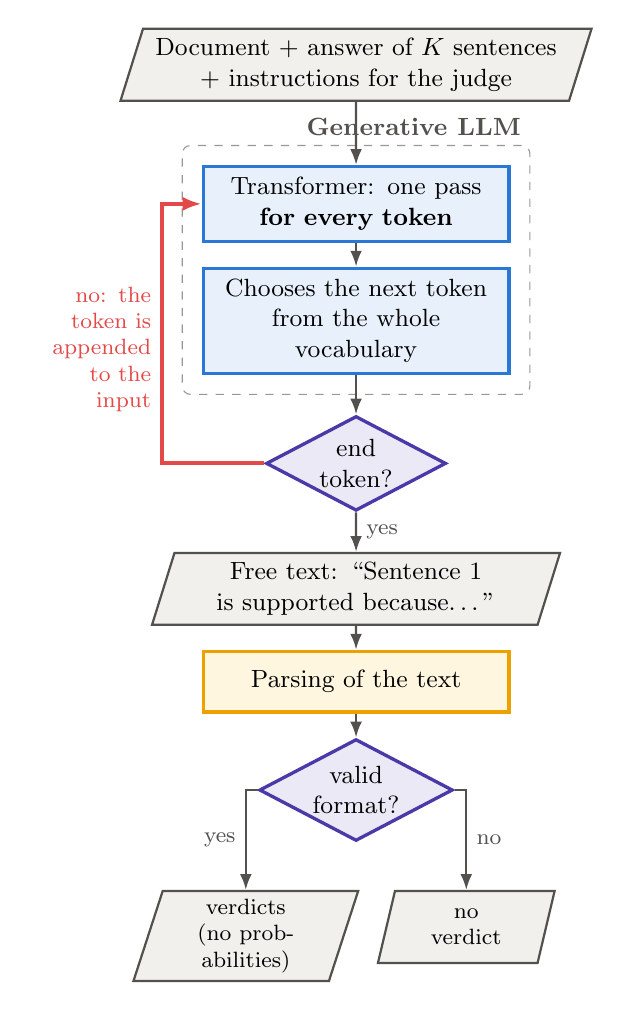
\begin{tikzpicture}[node distance=5mm]
  \node[io, text width=5.2cm] (in) {Document + answer of $K$ sentences\\+ instructions for the judge};
  \node[model, below=8mm of in] (t) {Transformer: one pass\\\textbf{for every token}};
  \node[model, below=3mm of t] (s) {Chooses the next token\\from the whole vocabulary};
  \begin{scope}[on background layer]
    \node[cluster, fit=(t)(s), label={[clusterlabel,anchor=south east]north east:Generative LLM}] (c) {};
  \end{scope}
  \node[decision, below=5mm of s] (d) {end\\token?};
  \node[io, below=5mm of d, text width=4.4cm] (txt) {Free text: ``Sentence 1\\is supported because\dots''};
  \node[post, below=3mm of txt] (p) {Parsing of the text};
  \node[decision, below=3mm of p] (f) {valid\\format?};
  \node[io, below=6mm of f, xshift=-14mm, font=\footnotesize, text width=1.9cm] (o1) {verdicts\\(no probabilities)};
  \node[io, below=6mm of f, xshift=14mm, font=\footnotesize, text width=1.6cm] (o2) {no\\verdict};
  \draw[arrow] (in) -- (t);
  \draw[arrow] (t) -- (s);
  \draw[arrow] (s) -- (d);
  \draw[loop] (d.west) -| node[pos=0.72, left, font=\footnotesize, text=loopRed, text width=1.45cm, align=right] {no: the\\token is\\appended\\to the input} ([xshift=-5mm]t.west) -- (t.west);
  \draw[arrow] (d) -- node[right, font=\footnotesize] {yes} (txt);
  \draw[arrow] (txt) -- (p);
  \draw[arrow] (p) -- (f);
  \draw[arrow] (f.west) -| node[pos=0.75, left, font=\footnotesize] {yes} (o1.north);
  \draw[arrow] (f.east) -| node[pos=0.75, right, font=\footnotesize] {no} (o2.north);
\end{tikzpicture}
\end{document}
